\section{Results}\label{sec:results}

This section answers the four research questions in turn. All test numbers are nDCG on uniformly exposed test data. Uniform data are used for validation and testing. The one exception is Coat's shipped propensities, which the dataset authors estimated from the uniform sample; Section~\ref{sec:res-ingredient} reports a refit with the estimator used on the other datasets. Otherwise nuisances are fitted on the exposed log, and every configuration and epoch is selected on validation data within each split. Table~\ref{tab:T4} gives the benchmark, with the mean and standard deviation over splits and the number of configurations searched for each method. Paired differences are per-user averages of the difference between two methods, taken over the users who appear in both test sets. They are given in units of $10^{-3}$ nDCG, with the 95\% confidence-interval half-width in brackets. A difference is called significant only when its Holm-adjusted p-value is below 0.05, and the Holm family is stated wherever a p-value is given. The evaluated users number 225 on Coat, 2,310 on Yahoo! R3, 8,321 on KuaiRand and 1,410 on KuaiRec. There are 10 splits on Coat and 5 on the other three datasets. The metric is nDCG@5 on Coat and Yahoo! R3, nDCG@10 on KuaiRand and nDCG@20 on KuaiRec.

\begin{table}[t]
\centering
\footnotesize
\caption{Main benchmark: mean test score over splits (sd over splits, ddof 0) and configuration count per method. Metric: nDCG@5 (Coat, Yahoo), nDCG@10 (KuaiRand), nDCG@20 (KuaiRec).}
\label{tab:T4}
\resizebox{\textwidth}{!}{%
\begin{tabular}{lrrrrrrrr}
\toprule
Method & \multicolumn{2}{c}{Coat} & \multicolumn{2}{c}{Yahoo} & \multicolumn{2}{c}{KuaiRand} & \multicolumn{2}{c}{KuaiRec} \\
 & mean (sd) & cfg & mean (sd) & cfg & mean (sd) & cfg & mean (sd) & cfg \\
\midrule
Obs & 0.5571 (0.0100) & 24 & 0.6585 (0.0058) & 16 & -- & -- & 0.6036 (0.0028) & 16 \\
Pop & 0.5367 (0.0095) & 1 & 0.5331 (0.0059) & 1 & -- & -- & 0.5766 (0.0023) & 1 \\
Impute & 0.5532 (0.0097) & 6 & 0.5162 (0.0044) & 2 & -- & -- & 0.6194 (0.0018) & 4 \\
IPS & 0.5510 (0.0224) & 720 & -- & -- & -- & -- & -- & -- \\
DR & 0.5459 (0.0244) & 1440 & 0.6567 (0.0063) & 512 & -- & -- & 0.6378 (0.0020) & 384 \\
DRUP & 0.5467 (0.0235) & 1440 & 0.6567 (0.0063) & 512 & -- & -- & 0.6378 (0.0019) & 384 \\
EASE & 0.5401 (0.0138) & 3 & -- & -- & -- & -- & -- & -- \\
GF-CF & 0.5512 (0.0124) & 4 & -- & -- & -- & -- & -- & -- \\
EASE-DR & 0.5564 (0.0141) & 90 & -- & -- & -- & -- & -- & -- \\
GF-CF-DR & 0.5598 (0.0084) & 120 & -- & -- & -- & -- & -- & -- \\
MF & 0.4780 (0.0168) & 18 & 0.5087 (0.0075) & 9 & 0.3705 (0.0008) & 6 & 0.6221 (0.0036) & 6 \\
IPS-MF & 0.4713 (0.0160) & 18 & 0.5125 (0.0059) & 9 & -- & -- & 0.6252 (0.0018) & 6 \\
DR-MF & 0.5237 (0.0111) & 18 & 0.5093 (0.0042) & 9 & 0.3608 (0.0067) & 6 & 0.6219 (0.0025) & 6 \\
BPR-MF & 0.5174 (0.0206) & 18 & 0.6461 (0.0042) & 9 & 0.4475 (0.0027) & 6 & 0.5963 (0.0028) & 6 \\
PDA & 0.5181 (0.0138) & 36 & 0.6514 (0.0051) & 18 & -- & -- & -- & -- \\
LightGCN & 0.5683 (0.0132) & 54 & 0.6708 (0.0061) & 36 & 0.4569 (0.0010) & 6 & 0.6085 (0.0028) & 36 \\
LightGCN-pt & 0.5389 (0.0107) & 54 & 0.5947 (0.0028) & 6 & 0.4061 (0.0014) & 6 & 0.6271 (0.0023) & 36 \\
r-AdjNorm & 0.5722 (0.0134) & 108 & 0.6742 (0.0047) & 72 & 0.4590 (0.0024) & 12 & 0.6083 (0.0031) & 12 \\
NAVIP & 0.5664 (0.0163) & 54 & 0.6701 (0.0039) & 36 & 0.4565 (0.0017) & 6 & 0.6186 (0.0024) & 6 \\
DR-LightGCN & 0.5724 (0.0205) & 54 & 0.5528 (0.0091) & 6 & -- & -- & 0.6212 (0.0071) & 6 \\
SimGCL & 0.5528 (0.0141) & 108 & 0.6348 (0.0048) & 12 & 0.4196 (0.0022) & 12 & 0.5637 (0.0031) & 12 \\
MACR & 0.5418 (0.0134) & 36 & 0.6221 (0.0038) & 18 & 0.4311 (0.0019) & 12 & 0.5816 (0.0033) & 12 \\
AdvInfoNCE-LGN & 0.5222 (0.0204) & 216 & 0.6477 (0.0048) & 16 & 0.4480 (0.0017) & 8 & 0.5776 (0.0036) & 8 \\
DR-JL & 0.4811 (0.0164) & 18 & 0.5225 (0.0043) & 9 & 0.3759 (0.0021) & 6 & 0.6332 (0.0026) & 6 \\
MRDR & 0.4869 (0.0187) & 18 & 0.5248 (0.0059) & 9 & -- & -- & 0.6328 (0.0020) & 6 \\
iALS & 0.5812 (0.0101) & 24 & 0.6625 (0.0043) & 12 & 0.4528 (0.0017) & 12 & 0.6133 (0.0027) & 12 \\
iALS-wide & 0.5869 (0.0118) & 18 & -- & -- & -- & -- & -- & -- \\
iALS-p (add prior) & 0.5984 (0.0121) & 90 & -- & -- & -- & -- & -- & -- \\
LightGCN-p (add prior) & 0.6020 (0.0148) & 108 & -- & -- & -- & -- & 0.6288 (0.0020) & 24 \\
DR-iALS & 0.5871 (0.0113) & 48 & -- & -- & -- & -- & -- & -- \\
DR-BPR-LGN & 0.5912 (0.0122) & 108 & -- & -- & -- & -- & -- & -- \\
DR-BPR-LGN-1 (Q, lrQ) & 0.5887 (0.0132) & 54 & -- & -- & -- & -- & -- & -- \\
DR-BPR-LGN-1 (Q) & -- & -- & 0.6837 (0.0057) & 36 & -- & -- & -- & -- \\
DR-BPR-LGN-p & 0.6039 (0.0139) & 108 & -- & -- & -- & -- & -- & -- \\
DR-BPR-LGN-p2 & 0.6046 (0.0177) & 108 & -- & -- & -- & -- & -- & -- \\
QP family (pooled) & 0.6015 (0.0162) & 324 & 0.6866 (0.0034) & 84 & 0.4613 (0.0024) & 30 & 0.6285 (0.0022) & 120 \\
control: shuffled Q & 0.5689 (0.0148) & 54 & 0.6689 (0.0054) & 12 & -- & -- & -- & -- \\
control: popularity Q & 0.5751 (0.0118) & 54 & 0.6550 (0.0046) & 12 & -- & -- & -- & -- \\
\bottomrule
\end{tabular}}
\par\smallskip\raggedright\footnotesize Pooled rows (QP family) pool the configurations of their jobs; a cell marked -- is not yet available (its inputs are not in results/ yet).
\end{table}


Table~\ref{tab:T5} reports the primary comparisons. P1 compares the strongest graph debiaser with LightGCN, and P2 compares a simple debiased prior with its backbone; both are reported on all four datasets. P3 compares the best refinement with the simple prior of the same learner, and P4 compares training-free doubly robust propagation with the best trained model on KuaiRec. P3 is reported on Coat and KuaiRec only, and P4 on KuaiRec only. The equivalence (TOST) margins are $\pm0.010$ on Coat and Yahoo! R3 and $\pm0.003$ on KuaiRand and KuaiRec. They were declared before the analysis but have not yet been checked against published effect sizes, so they are provisional.

\subsection{Effects of evaluation choices (RQ1)}\label{sec:res-eval}

Selecting on the test split inflates the reported scores, and the inflation differs between methods. Across the trained methods in the sensitivity analysis, the per-split test oracle exceeds the validation-selected score by a mean of $+0.0207$ on Coat (range $+0.0097$ to $+0.0302$), $+0.0044$ on Yahoo! R3 (range $+0.0015$ to $+0.0088$), $+0.0012$ on KuaiRand (range $+0.0005$ to $+0.0022$) and $+0.0009$ on KuaiRec (range $+0.0000$ to $+0.0028$). On Coat the inflation is largest for DR-JL ($+0.0302$) and smallest for iALS ($+0.0097$), while LightGCN inflates by $+0.0241$. This is enough to change an order. Under validation selection iALS scores $0.5812$ and LightGCN $0.5683$. Under the per-split test oracle the scores are $0.5909$ for iALS and $0.5924$ for LightGCN. The configuration-level oracle, which picks one configuration by its mean test score, keeps the validation order, with $0.5843$ for iALS and $0.5807$ for LightGCN. A comparison made on test data can therefore change sign, and the two kinds of test oracle do not agree on Coat.

The searched grids differ in size, from 6 configurations for several KuaiRand and KuaiRec baselines to 324 for the QP family on Coat. To measure how much this matters, we drew 1,000 random subgrids of $k_\mathrm{min}$ configurations for each comparison and counted how often its sign changed (Table~\ref{tab:T7}). Flips are common for comparisons whose effects are near zero. The QP family against LightGCN-p changes sign in 35.3\% of the subgrids on Coat and 30.9\% on KuaiRec. The largest instability is DRUP against DR-JL on KuaiRec. At $k_\mathrm{min}=6$, 78.4\% of the subgrids flip the sign, and the split-mean difference at matched budget is $-14.90$, while the full-grid per-user difference is $+4.38$ [2.21]. DRUP is training-free but searches 384 configurations on KuaiRec, against 6 for DR-JL, so its advantage over DR-JL depends on the budget granted to each method. The matched-budget values in Table~\ref{tab:T5} are split means and carry no test.

The weighting unit can also change a sign. For DR-LightGCN against LightGCN on Coat, the split-mean difference at matched budget ($k=54$) is $+4.11$, while the per-user paired difference is $-0.65$ [30.16]. Every test in this paper uses the per-user unit. The split-mean values are reported only as matched-budget descriptions, and they are not tested.

Retraining the selected configurations with seeds 1 to 3 changes two main-run conclusions (Table~\ref{tab:T5} and the seed summary). On Coat, \qp{} against iALS is $+20.02$ [19.74] in the main run (p$_\mathrm{Holm}$ = 0.0469, in a family of eight baselines). Over seeds 1 to 3 the difference is $+3.39$ [20.70] (p$_\mathrm{Holm}$ = 0.747, in a family of two), which is not significant. On KuaiRec the main-run deficits of \qp{} against DR-JL and MRDR, $-4.56$ [2.24] and $-4.34$ [2.16], shrink over seeds 1 to 3 to $-1.03$ [1.64] (p$_\mathrm{Holm}$ = 0.2213) and $-1.56$ [1.47] (p$_\mathrm{Holm}$ = 0.0760). The gains on Yahoo! R3 and KuaiRand survive the reseeding: \qp{} exceeds r-AdjNorm by $+14.76$ [5.23] on Yahoo! R3 and by $+2.31$ [1.23] on KuaiRand, with p$_\mathrm{Holm}$ below 0.001 and 0.0002 respectively. The seed-to-seed standard deviation of \qp{} on Coat (0.0049) is larger than that of iALS (0.0029), so the main-run Coat result is a single-run result.

Changing the metric changes 3 of the 14 pairwise conclusions in Table~\ref{tab:T7}: the Coat comparisons of DR-LightGCN with LightGCN and of the QP family with LightGCN-p, and the KuaiRec comparison of DR-LightGCN with LightGCN. The alternative metric is nDCG@10 on Coat and Yahoo! R3, nDCG@20 on KuaiRand and nDCG@50 on KuaiRec. Of the 14 conclusions, 7 are significant at p$_\mathrm{Holm}$ < 0.05 in the main run. Their signs survive the per-split test oracle in 12 cases, the configuration-level oracle in 11, matched budget in 13 and the alternative metric in 11.

\begin{table}[t]
\centering
\footnotesize
\caption{Sensitivity of the primary conclusions to evaluation choices (A1, A2). A check mark means the sign of the difference (and, for Main, significance at $p_\mathrm{Holm}<0.05$) survives the choice; the value is the difference $\times10^{3}$ under that choice. Main: per-user difference. Oracle, configuration-oracle and matched-budget columns: split-mean difference, compared in sign with the split-mean validation-selected difference.}
\label{tab:T7}
\resizebox{\textwidth}{!}{%
\begin{tabular}{lllllllrrlll}
\toprule
Dataset & Fam. & Comparison & Main (Holm) & Test oracle & Config.\ oracle & Matched $k$ & $k_\mathrm{min}$ & Flip share & Seeds & NB & Alt.\ metric \\
\midrule
Coat & P1 & DR-LightGCN -- LightGCN & $\times$ -0.65 & $\checkmark$ +1.23 & $\times$ -6.63 & $\checkmark$ +4.11 & 54 & 0.0\% & n/a & $\times$ & $\times$ \\
Coat & P2 & iALS-p (add prior) -- iALS & $\times$ +16.82 & $\checkmark$ +31.66 & $\checkmark$ +21.23 & $\checkmark$ +16.12 & 24 & 0.0\% & n/a & $\times$ & $\checkmark$ \\
Coat & P2 & LightGCN-p (add prior) -- LightGCN & $\checkmark$ +31.98 & $\checkmark$ +27.74 & $\checkmark$ +28.27 & $\checkmark$ +34.12 & 54 & 0.0\% & n/a & $\times$ & $\checkmark$ \\
Coat & P3 & QP family (pooled) -- LightGCN-p (add prior) & $\times$ +0.05 & $\times$ +2.17 & $\times$ +1.42 & $\checkmark$ -0.36 & 108 & 35.3\% & n/a & $\times$ & $\times$ \\
Coat & P3 & DR-iALS -- iALS-p (add prior) & $\times$ -10.22 & $\checkmark$ -24.87 & $\checkmark$ -13.87 & $\checkmark$ -11.21 & 48 & 0.0\% & n/a & $\times$ & $\checkmark$ \\
Yahoo & P1 & r-AdjNorm -- LightGCN & $\checkmark$ +4.10 & $\checkmark$ +2.35 & $\checkmark$ +0.57 & $\checkmark$ +2.87 & 36 & 2.4\% & $\checkmark$ & $\times$ & $\checkmark$ \\
Yahoo & P2 & LightGCN-p (add prior) -- LightGCN & $\times$ -1.43 & $\checkmark$ -0.07 & $\checkmark$ -1.11 & $\checkmark$ -2.16 & 24 & 0.0\% & n/a & $\times$ & $\checkmark$ \\
KuaiRand & P1 & r-AdjNorm -- LightGCN & $\checkmark$ +1.99 & $\checkmark$ +1.76 & $\checkmark$ +1.80 & $\checkmark$ +1.23 & 6 & 9.4\% & $\checkmark$ & $\times$ & $\checkmark$ \\
KuaiRand & P2 & LightGCN-p (add prior) -- LightGCN & $\times$ -0.81 & $\checkmark$ -0.03 & $\checkmark$ -0.84 & $\checkmark$ -0.79 & 6 & 7.1\% & n/a & $\times$ & $\checkmark$ \\
KuaiRec & P1 & DR-LightGCN -- LightGCN & $\checkmark$ +13.17 & $\checkmark$ +14.69 & $\checkmark$ +12.44 & $\checkmark$ +12.97 & 6 & 0.0\% & n/a & $\times$ & $\times$ \\
KuaiRec & P2 & LightGCN-p (add prior) -- LightGCN & $\checkmark$ +21.22 & $\checkmark$ +20.02 & $\checkmark$ +20.00 & $\checkmark$ +20.25 & 24 & 0.0\% & n/a & $\checkmark$ & $\checkmark$ \\
KuaiRec & P2 & iALS-p (add prior) -- iALS & $\checkmark$ +14.74 & $\checkmark$ +14.00 & $\checkmark$ +14.00 & $\checkmark$ +16.89 & 8 & 0.0\% & n/a & $\checkmark$ & $\checkmark$ \\
KuaiRec & P3 & QP family (pooled) -- LightGCN-p (add prior) & $\times$ -0.32 & $\times$ +0.32 & $\times$ +0.46 & $\checkmark$ -0.12 & 24 & 30.9\% & n/a & $\times$ & $\checkmark$ \\
KuaiRec & P4 & DRUP -- DR-JL & $\checkmark$ +4.38 & $\checkmark$ +5.48 & $\checkmark$ +5.45 & $\times$ -14.90 & 6 & 78.4\% & n/a & $\times$ & $\checkmark$ \\
\bottomrule
\end{tabular}}
\par\smallskip\raggedright\footnotesize Flip share: fraction of 1,000 random subgrids of $k_\mathrm{min}$ configurations per method whose sign differs from the full grid. Alt.\ metric: nDCG@10 (Coat, Yahoo), nDCG@20 (KuaiRand), nDCG@50 (KuaiRec), on the stored selections.
\end{table}


\begin{figure}[t]
\centering
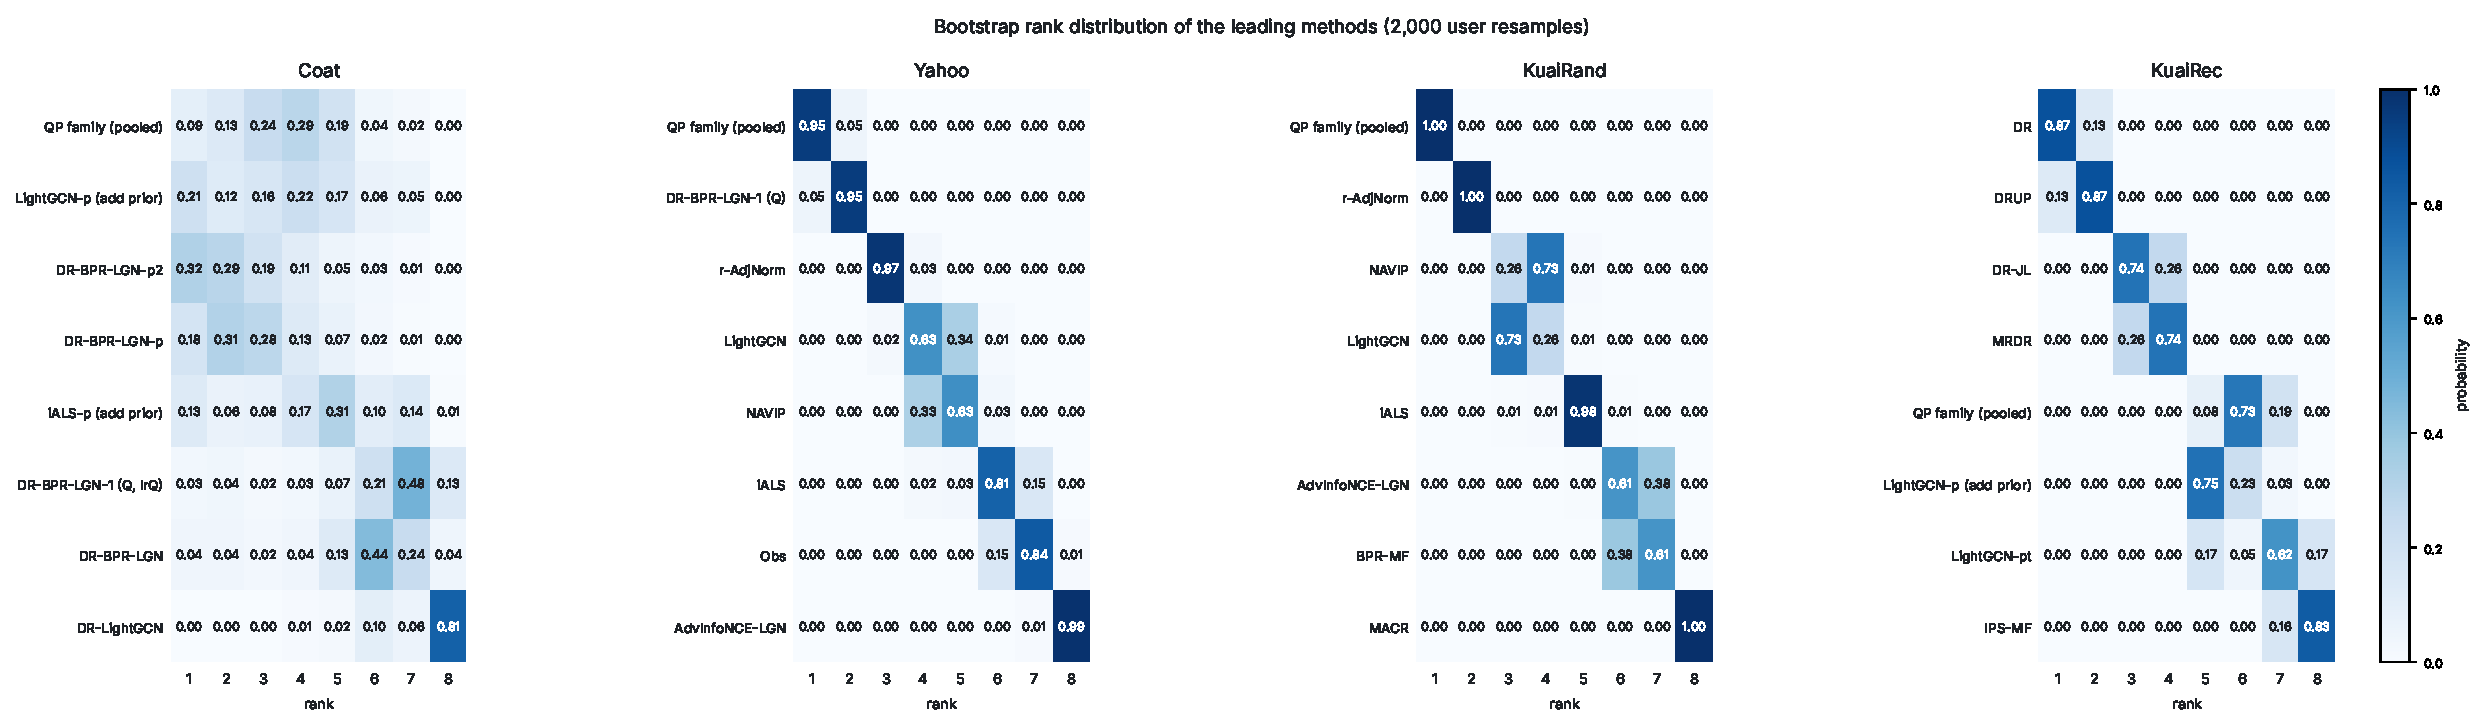
\includegraphics[width=\linewidth]{figs/rank_distribution}
\caption{Bootstrap rank distributions over 2,000 user resamples. For each dataset the rows are the eight methods with the highest mean validation score, excluding control rows, and the columns are the rank by mean test score (1 is best). On Coat the splits are resampled together with the users. Each cell gives the probability of that rank.}
\label{fig:rank}
\end{figure}

The bootstrap ranks (Figure~\ref{fig:rank}) show how stable the leader is. On Yahoo! R3 the QP family ranks first in 95.0\% of user resamples, and on KuaiRand in 99.8\%. On KuaiRec, DR and DRUP have the same mean score (0.6378) and exchange first place, with probabilities 0.873 and 0.127. The bootstrap therefore cannot separate them. On Coat no method is a stable leader. The most frequent first place is DR-BPR-LGN-p2, with probability 0.319, and the QP family ranks first with probability 0.090.

\subsection{What graph debiasing adds over an equally tuned backbone (RQ2)}\label{sec:res-debias}

On Coat the graph debiasers are not separated from LightGCN. The three with stored Coat results differ from it by $+3.76$ [5.74] (r-AdjNorm), $-1.59$ [10.13] (NAVIP) and $-0.65$ [30.16] (DR-LightGCN), and none of these is significant. Under the provisional margin of $\pm0.010$, the r-AdjNorm difference is equivalent to zero (TOST p = 0.017), while the NAVIP difference (p = 0.0515) and the DR-LightGCN difference (p = 0.271) are not. The minimum detectable difference for the primary comparison P1 on Coat is $43.07$ ($\times10^{-3}$), so the study cannot exclude a gain of that size for DR-LightGCN. On Coat, iALS differs from LightGCN by $+12.01$ [16.12] (p = 0.143, not significant).

On Yahoo! R3, r-AdjNorm is $+4.10$ [3.29] above LightGCN (p = 0.015, p$_\mathrm{Holm}$ = 0.029 in the two-comparison primary family). Adjusting over all comparisons with LightGCN in the appendix gives p$_\mathrm{Holm}$ = 0.073, and the Nadeau-Bengio correction for overlapping splits gives p$_\mathrm{Holm}$ = 0.883. On KuaiRand, r-AdjNorm is $+1.99$ [1.02] above LightGCN (p$_\mathrm{Holm}$ < 0.001). This difference lies inside the provisional margin of $\pm0.003$ (TOST p = 0.026), and the Nadeau-Bengio correction gives p$_\mathrm{Holm}$ = 1.000. Across Coat, Yahoo! R3 and KuaiRand, then, the best graph debiaser adds at most $+4.10$ ($\times10^{-3}$) nDCG over the equally tuned backbone, and the Nadeau-Bengio correction removes its significance.

KuaiRec, whose test matrix is fully observed, differs. DR-LightGCN is $+13.17$ [3.31] above LightGCN (p$_\mathrm{Holm}$ < 0.001) and NAVIP is $+10.41$ [1.82] above it (appendix). Under the Nadeau-Bengio correction the DR-LightGCN difference has p$_\mathrm{Holm}$ = 0.787. The pointwise LightGCN-pt, which has no debiasing, is $+19.59$ [4.55] above the BPR backbone. On KuaiRec, then, the change of loss contributes more than any graph debiaser does. The training-free operators are stronger still on this dataset (Section~\ref{sec:res-walk}).

The re-implementation of AdvInfoNCE is below LightGCN on all four datasets: $-46.47$ [25.16] on Coat, $-21.08$ [7.78] on Yahoo! R3, $-8.86$ [2.50] on KuaiRand and $-28.42$ [6.46] on KuaiRec, each significant under the appendix Holm adjustment. SimGCL and MACR are below LightGCN on all four datasets and significantly so on Yahoo! R3, KuaiRand and KuaiRec. On Coat, their differences ($-17.49$ [23.88] and $-29.43$ [24.60]) are not significant. These comparisons use our implementations, which are described in the protocol section.

Table~\ref{tab:T5} gives the primary comparisons with their Nadeau-Bengio columns. Under that correction, none of the four P1 comparisons is significant. The two P2 comparisons on KuaiRec remain significant, with p$_\mathrm{NB,Holm}$ of 0.009 for LightGCN-p and 0.043 for iALS-p. The P4 comparison, DRUP against DR-JL, is significant under the per-user test ($+4.38$ [2.21], p$_\mathrm{Holm}$ < 0.001) but not under the correction (p$_\mathrm{NB,Holm}$ = 0.426).

\begin{table}[t]
\centering
\footnotesize
\caption{Primary comparisons P1--P4 (Section 2.3): paired per-user differences, tests, MDE, TOST at the margins of Section 2.3, and the matched-budget difference at $k=k_\mathrm{min}$.}
\label{tab:T5}
\resizebox{\textwidth}{!}{%
\begin{tabular}{llllrrrrlrl}
\toprule
Dataset & Fam. & Comparison ($A-B$) & Diff.\ $\times10^{3}$ [95\% CI] & $p$ & $p_\mathrm{Holm}$ & $p_\mathrm{NB,Holm}$ & MDE $\times10^{3}$ & TOST at margin & Matched-$k$ diff $\times10^{3}$ & Seeds 1--3 diff $\times10^{3}$ \\
\midrule
Coat & P1 & DR-LightGCN -- LightGCN & -0.65 [30.16] & 0.966 & 1.000 & 1.000 & 43.07 & no ($p$=0.271) & +4.11 & -- \\
Coat & P2 & iALS-p (add prior) -- iALS & +16.82 [18.04] & 0.068 & 0.270 & 1.000 & 25.76 & no ($p$=0.771) & +16.12 & -- \\
Coat & P2 & LightGCN-p (add prior) -- LightGCN & +31.98 [20.65] & 0.003 & 0.013 & 1.000 & 29.48 & no ($p$=0.981) & +34.12 & -- \\
Coat & P3 & QP family (pooled) -- LightGCN-p (add prior) & +0.05 [8.29] & 0.991 & 1.000 & 1.000 & 11.83 & yes ($p$=0.009) & -0.36 & -- \\
Coat & P3 & DR-iALS -- iALS-p (add prior) & -10.22 [15.96] & 0.208 & 0.625 & 1.000 & 22.79 & no ($p$=0.511) & -11.21 & -- \\
Yahoo & P1 & r-AdjNorm -- LightGCN & +4.10 [3.29] & 0.015 & 0.029 & 0.883 & 4.70 & yes ($p$=0.000) & +2.87 & +5.26 ($p$=0.000) \\
Yahoo & P2 & LightGCN-p (add prior) -- LightGCN & -1.43 [3.93] & 0.475 & 0.475 & 0.883 & 5.62 & yes ($p$=0.000) & -2.16 & -- \\
KuaiRand & P1 & r-AdjNorm -- LightGCN & +1.99 [1.02] & 0.000 & 0.000 & 1.000 & 1.46 & yes ($p$=0.026) & +1.23 & +2.56 ($p$=0.000) \\
KuaiRand & P2 & LightGCN-p (add prior) -- LightGCN & -0.81 [1.33] & 0.234 & 0.234 & 1.000 & 1.90 & yes ($p$=0.001) & -0.79 & -- \\
KuaiRec & P1 & DR-LightGCN -- LightGCN & +13.17 [3.31] & 0.000 & 0.000 & 0.787 & 4.74 & no ($p$=1.000) & +12.97 & -- \\
KuaiRec & P2 & LightGCN-p (add prior) -- LightGCN & +21.22 [2.86] & 0.000 & 0.000 & 0.009 & 4.09 & no ($p$=1.000) & +20.25 & -- \\
KuaiRec & P2 & iALS-p (add prior) -- iALS & +14.74 [3.43] & 0.000 & 0.000 & 0.043 & 4.90 & no ($p$=1.000) & +16.89 & -- \\
KuaiRec & P3 & QP family (pooled) -- LightGCN-p (add prior) & -0.32 [0.50] & 0.211 & 0.211 & 0.871 & 0.72 & yes ($p$=0.000) & -0.12 & -- \\
KuaiRec & P4 & DRUP -- DR-JL & +4.38 [2.21] & 0.000 & 0.000 & 0.426 & 3.15 & no ($p$=0.890) & -14.90 & -- \\
\bottomrule
\end{tabular}}
\par\smallskip\raggedright\footnotesize Margins are the provisional values of Section 2.3 (TODO-L2 not yet closed). Seeds column: only comparisons whose baselines are in results/v4/seeds_*.json.
\end{table}


\subsection{Which ingredient carries the gain (RQ3)}\label{sec:res-ingredient}

The simple prior is the additive imputation $\hat\mu+b_u+b_i$, fitted once on the exposed log with inverse-propensity weights and added to the score as an offset. Within a user its ranking is the ranking of the item term $b_i$. Used as an offset on LightGCN (LightGCN-p), it gives $+31.98$ [20.65] on Coat (p$_\mathrm{Holm}$ = 0.013 in the primary family of Table~\ref{tab:T5}; 0.046 in the family of Table~\ref{tab:T9}), and $+21.22$ [2.86] on KuaiRec (p$_\mathrm{Holm}$ < 0.001). On Yahoo! R3 it gives $-1.43$ [3.93] (p$_\mathrm{Holm}$ = 0.475), and on KuaiRand $-0.81$ [1.33] (p$_\mathrm{Holm}$ = 0.234). The offset-only summary uses a different Holm family and reports 0.008 for Coat and 0.468 for KuaiRand. The offset helps on Coat and KuaiRec and not on Yahoo! R3 or KuaiRand. The tests here do not explain this pattern.

Table~\ref{tab:T9} separates the additive prior into its parts: the IPS weighting, the item term, and popularity. Removing the IPS weights does not reduce the gain. On KuaiRec, the unweighted prior added to iALS gives $+22.79$ [4.04] over iALS, and it exceeds the weighted prior by $+8.05$ [2.06] (p$_\mathrm{Holm}$ < 0.001). On Coat the unweighted prior is above the weighted one by $+6.27$ [6.97] for iALS and $+4.01$ [10.01] for LightGCN, neither significant. Popularity does not reproduce the effect on KuaiRec: its offset adds $+1.06$ [2.46] to iALS (p$_\mathrm{Holm}$ = 1.000), against $+14.74$ [3.43] for the weighted prior. Replacing the item term by a random permutation across items removes the KuaiRec gain and reverses it, with $-112.07$ [9.39] against iALS (p$_\mathrm{Holm}$ < 0.001). On Coat the same permutation gives $-14.06$ [18.53] for iALS and $-12.95$ [24.18] for LightGCN, neither significant, so the Coat result does not isolate the item term. The lowest offset weight of the grid was selected in all five KuaiRec splits for the shuffled item term, so the reported harm is an upper bound under that grid.

\begin{table}[t]
\centering
\footnotesize
\caption{Prior anatomy (X1). Test nDCG of iALS-p and LightGCN-p under four additive-imputation variants, and of the prior alone on all four datasets.}
\label{tab:T9}
\resizebox{\textwidth}{!}{%
\begin{tabular}{llrrrrr}
\toprule
Dataset & Learner / prior & nDCG (mean $\pm$ sd) & $\Delta$ vs no prior $\times10^{3}$ [CI] & $p_\mathrm{Holm}$ & $\Delta$ vs add $\times10^{3}$ [CI] & $p_\mathrm{Holm}$ \\
\midrule
Coat & iALS (no prior) & 0.5812 $\pm$ 0.0107 & -- & -- & -- & -- \\
Coat & iALS-p, add (IPS-fitted) & 0.5984 $\pm$ 0.0128 & +16.82 [18.04] & 0.811 & -- & -- \\
Coat & iALS-p, add, no IPS & 0.6044 $\pm$ 0.0115 & +23.08 [18.24] & 0.187 & +6.27 [6.97] & 0.856 \\
Coat & iALS-p, pop & 0.5832 $\pm$ 0.0238 & +1.67 [16.11] & 1.000 & -15.15 [15.39] & 0.698 \\
Coat & iALS-p, shuffled item bias & 0.5683 $\pm$ 0.0175 & -14.06 [18.53] & 1.000 & -30.87 [22.75] & 0.120 \\
Coat & LightGCN (no prior) & 0.5683 $\pm$ 0.0139 & -- & -- & -- & -- \\
Coat & LightGCN-p, add (IPS-fitted) & 0.6020 $\pm$ 0.0156 & +31.98 [20.65] & 0.046 & -- & -- \\
Coat & LightGCN-p, add, no IPS & 0.6052 $\pm$ 0.0145 & +36.00 [16.88] & $<$0.001 & +4.01 [10.01] & 1.000 \\
Coat & LightGCN-p, pop & 0.5835 $\pm$ 0.0233 & +15.63 [10.68] & 0.069 & -16.36 [19.52] & 1.000 \\
Coat & LightGCN-p, shuffled item bias & 0.5527 $\pm$ 0.0095 & -12.95 [24.18] & 1.000 & -44.93 [29.53] & 0.051 \\
KuaiRec & iALS (no prior) & 0.6133 $\pm$ 0.0030 & -- & -- & -- & -- \\
KuaiRec & iALS-p, add (IPS-fitted) & 0.6273 $\pm$ 0.0018 & +14.74 [3.43] & $<$0.001 & -- & -- \\
KuaiRec & iALS-p, add, no IPS & 0.6350 $\pm$ 0.0021 & +22.79 [4.04] & $<$0.001 & +8.05 [2.06] & $<$0.001 \\
KuaiRec & iALS-p, pop & 0.6144 $\pm$ 0.0028 & +1.06 [2.46] & 1.000 & -13.68 [3.31] & $<$0.001 \\
KuaiRec & iALS-p, shuffled item bias & 0.4993 $\pm$ 0.0032 & -112.07 [9.39] & $<$0.001 & -126.82 [9.29] & $<$0.001 \\
KuaiRec & LightGCN (no prior) & 0.6085 $\pm$ 0.0031 & -- & -- & -- & -- \\
KuaiRec & LightGCN-p, add (IPS-fitted) & 0.6288 $\pm$ 0.0023 & +21.22 [2.86] & $<$0.001 & -- & -- \\
Coat & prior alone, add (IPS-fitted) & 0.5585 $\pm$ 0.0105 & -- & -- & -- & -- \\
Coat & prior alone, add, no IPS & 0.5574 $\pm$ 0.0107 & -- & -- & -2.09 [8.46] & 1.000 \\
Coat & prior alone, pop & 0.5367 $\pm$ 0.0100 & -- & -- & -19.40 [27.79] & 1.000 \\
Coat & prior alone, shuffled item bias & 0.3572 $\pm$ 0.0125 & -- & -- & -203.62 [51.90] & $<$0.001 \\
Coat & prior alone, user only (b\_i = 0) & 0.3497 $\pm$ 0.0152 & -- & -- & -207.15 [49.91] & $<$0.001 \\
Yahoo & prior alone, add (IPS-fitted) & 0.5243 $\pm$ 0.0050 & -- & -- & -- & -- \\
Yahoo & prior alone, add, no IPS & 0.5237 $\pm$ 0.0055 & -- & -- & -1.09 [3.98] & 1.000 \\
Yahoo & prior alone, pop & 0.5331 $\pm$ 0.0065 & -- & -- & +8.90 [14.93] & 1.000 \\
Yahoo & prior alone, shuffled item bias & 0.3446 $\pm$ 0.0056 & -- & -- & -177.98 [17.37] & $<$0.001 \\
Yahoo & prior alone, user only (b\_i = 0) & 0.3767 $\pm$ 0.0051 & -- & -- & -144.74 [17.38] & $<$0.001 \\
KuaiRand & prior alone, add (IPS-fitted) & 0.3637 $\pm$ 0.0013 & -- & -- & -- & -- \\
KuaiRand & prior alone, add, no IPS & 0.3837 $\pm$ 0.0023 & -- & -- & +19.90 [2.45] & $<$0.001 \\
KuaiRand & prior alone, pop & 0.4204 $\pm$ 0.0021 & -- & -- & +56.41 [5.19] & $<$0.001 \\
KuaiRand & prior alone, shuffled item bias & 0.3257 $\pm$ 0.0018 & -- & -- & -39.12 [5.64] & $<$0.001 \\
KuaiRand & prior alone, user only (b\_i = 0) & 0.3259 $\pm$ 0.0011 & -- & -- & -38.84 [5.53] & $<$0.001 \\
KuaiRec & prior alone, add (IPS-fitted) & 0.6216 $\pm$ 0.0016 & -- & -- & -- & -- \\
KuaiRec & prior alone, add, no IPS & 0.6367 $\pm$ 0.0022 & -- & -- & +15.16 [1.68] & $<$0.001 \\
KuaiRec & prior alone, pop & 0.5766 $\pm$ 0.0026 & -- & -- & -45.70 [4.25] & $<$0.001 \\
KuaiRec & prior alone, shuffled item bias & 0.0398 $\pm$ 0.0007 & -- & -- & -582.01 [10.19] & $<$0.001 \\
KuaiRec & prior alone, user only (b\_i = 0) & 0.0686 $\pm$ 0.0010 & -- & -- & -554.01 [10.16] & $<$0.001 \\
\bottomrule
\end{tabular}}
\par\smallskip\raggedright\footnotesize $\Delta$ = per-user paired difference (mean over splits), $\times10^{3}$, [half-width of the 95\% CI]. No-prior references: stored iALS and LightGCN. The add row is the IPS-fitted additive prior. $p_\mathrm{Holm}$ over all paired tests of this table. user only (b\_i = 0) gives the same score to every item for a given user, so its ranking is decided by tie-breaking. Coat LightGCN-p and iALS-p use 10 splits, KuaiRec 5. Rows absent from the table were not run (only the prior-alone rows exist for those priors).
\end{table}


The training-free rows of Table~\ref{tab:T9} show the prior alone, with no learner. On KuaiRec the unweighted prior alone reaches $0.6367$, and the weighted prior alone $0.6216$. Popularity alone reaches $0.5766$. On KuaiRand the picture is different: popularity alone ($0.4204$) exceeds the weighted prior alone ($0.3637$) by $+56.41$ [5.19] (p$_\mathrm{Holm}$ < 0.001), and the unweighted prior alone ($0.3837$) exceeds the weighted one by $+19.90$ [2.45]. On Coat and Yahoo! R3, popularity alone is not significantly different from the weighted prior alone. The paired tests in the table are between the variants of the prior. No paired test of the prior alone against the training-free DRUP operator is in the result files, so the $0.0011$ gap between the unweighted prior alone and DRUP on KuaiRec is reported as a difference of means only.

The weights on the sampled negatives form the second ingredient. On Yahoo! R3 the weights without the offset (DR-BPR-LGN-1) exceed LightGCN-p by $+15.15$ [5.84] (p$_\mathrm{Holm}$ < 0.001), and the QP family exceeds LightGCN-p on KuaiRand by $+4.74$ [1.54] (p$_\mathrm{Holm}$ < 0.001). A shuffled Q removes the Yahoo! R3 gain, with $-1.01$ [3.20] against LightGCN (p$_\mathrm{Holm}$ = 0.534). On Coat, shuffled Q gives $+0.97$ [5.50] against LightGCN (p$_\mathrm{Holm}$ = 0.73), while popularity weights give $+6.91$ [6.04] (p$_\mathrm{Holm}$ = 0.0505, not significant). On Yahoo! R3, popularity weights are significantly below LightGCN ($-15.91$ [6.06], p$_\mathrm{Holm}$ < 0.001). On KuaiRand the validated combination selected $\beta=0$ in four of five splits, so the gain there comes from the weights.

The refinements built on the prior do not improve on it where the prior is tested. On Coat, the QP family is equivalent to LightGCN-p within $\pm0.010$ ($+0.05$ [8.29], TOST p = 0.009). The largest refinement difference from LightGCN-p is $+3.27$ [6.94] (DR-BPR-LGN-p2), which is not significant. The Q-only variants are $-8.02$ [18.85] and $-10.79$ [19.26] below it. On iALS, DR-iALS is $-10.22$ [15.96] against iALS-p (p$_\mathrm{Holm}$ = 0.208). On KuaiRec the QP family is $-0.32$ [0.50] against LightGCN-p (p$_\mathrm{Holm}$ = 0.211, equivalent within $\pm0.003$). Every refinement in the study is below DRUP ($0.6378$) on KuaiRec. The DRGP refinement, which uses a leave-edge-out DR-fitted prior, reaches $0.6318$, which is $-5.58$ [1.90] against DRUP (p$_\mathrm{Holm}$ < 0.0001). These DRGP results are stage-1 results without seeds, and DRGP was run on Coat and KuaiRec only. Its Coat score of $0.5992$ is $-0.13$ [15.11] against \qp{} (p$_\mathrm{Holm}$ = 1.000). A validated ensemble of \qp{} and DRUP selects one component in most splits and does not add to either: DRUP in four of five KuaiRec splits and \qp{} in nine of ten Coat splits. On KuaiRec the ensemble is $-0.18$ [0.19] against DRUP (p$_\mathrm{Holm}$ = 0.0664), and on Coat it is $+1.79$ [2.39] against \qp{} (p$_\mathrm{Holm}$ = 0.1421).

\begin{table}[t]
\centering
\footnotesize
\caption{Refinement family against the simple debiased prior of the same learner, and the shuffled and popularity controls against the backbone.}
\label{tab:T6}
\resizebox{\textwidth}{!}{%
\begin{tabular}{lllrrlrrl}
\toprule
Dataset & Family & Method & Mean & Cfg & Versus & Diff.\ $\times10^{3}$ [95\% CI] & $p_\mathrm{Holm}$ & TOST (Coat: exclusion, not equivalence) \\
\midrule
Coat & refinement vs simple prior & DR-BPR-LGN & 0.5912 & 108 & LightGCN-p (add prior) & -8.02 [18.85] & 1.000 & does not exclude \\
Coat & refinement vs simple prior & DR-BPR-LGN-1 (Q-only) & 0.5887 & 54 & LightGCN-p (add prior) & -10.79 [19.26] & 1.000 & does not exclude \\
Coat & refinement vs simple prior & DR-BPR-LGN-p & 0.6039 & 108 & LightGCN-p (add prior) & +2.09 [6.48] & 1.000 & excludes $\lvert d\rvert>0.010$ \\
Coat & refinement vs simple prior & DR-BPR-LGN-p2 & 0.6046 & 108 & LightGCN-p (add prior) & +3.27 [6.94] & 1.000 & excludes $\lvert d\rvert>0.010$ \\
Coat & refinement vs simple prior & QP family (pooled) & 0.6015 & 324 & LightGCN-p (add prior) & +0.05 [8.29] & 1.000 & excludes $\lvert d\rvert>0.010$ \\
Coat & refinement vs simple prior (iALS) & DR-iALS & 0.5871 & 48 & iALS-p (add prior) & -10.22 [15.96] & 0.208 & does not exclude \\
Coat & controls vs backbone & control: shuffled Q & 0.5689 & 54 & LightGCN & +0.97 [5.50] & 0.730 & excludes $\lvert d\rvert>0.010$ \\
Coat & controls vs backbone & control: popularity Q & 0.5751 & 54 & LightGCN & +6.91 [6.04] & 0.050 & does not exclude \\
Yahoo & refinement vs simple prior & DR-BPR-LGN-1 (Q-only) & 0.6837 & 36 & LightGCN-p (add prior) & +15.15 [5.84] & $<$0.001 & no \\
Yahoo & refinement vs simple prior & QP family (pooled) & 0.6866 & 84 & LightGCN-p (add prior) & +18.20 [5.64] & $<$0.001 & no \\
Yahoo & controls vs backbone & control: shuffled Q & 0.6689 & 12 & LightGCN & -1.01 [3.20] & 0.534 & yes \\
Yahoo & controls vs backbone & control: popularity Q & 0.6550 & 12 & LightGCN & -15.91 [6.06] & $<$0.001 & no \\
KuaiRand & refinement vs simple prior & QP family (pooled) & 0.4613 & 30 & LightGCN-p (add prior) & +4.74 [1.54] & $<$0.001 & no \\
KuaiRec & refinement vs simple prior & QP family (pooled) & 0.6285 & 120 & LightGCN-p (add prior) & -0.32 [0.50] & 0.211 & yes \\
\bottomrule
\end{tabular}}
\par\smallskip\raggedright\footnotesize Holm within each family and dataset. Rows are missing where the simple prior has not been run for that dataset.
\end{table}


Two checks on the prior concern its inputs. The first is the propensity model. Coat's shipped propensities were estimated by the dataset authors from the uniform sample, so we refitted them with the estimator used on the other three datasets. Table~\ref{tab:T10} shows that this changes little. The estimated-minus-shipped difference is $+2.63$ [5.27] for iALS-p and $+1.64$ [10.30] for LightGCN-p, and the imputation alone changes by $-1.14$ [7.26]. None is significant. The gain over the no-prior reference remains: $+19.44$ [18.66] for iALS-p and $+33.62$ [16.72] for LightGCN-p. The estimated-propensity run of LightGCN was not carried out.

\begin{table}[t]
\centering
\footnotesize
\caption{Coat with estimated propensities (X2): --prop pop versus the shipped propensities.}
\label{tab:T10}
\resizebox{\textwidth}{!}{%
\begin{tabular}{llrrrrr}
\toprule
Method & Propensities & nDCG (mean $\pm$ sd) & $\Delta$ vs no-prior $\times10^{3}$ [CI] & $p_\mathrm{Holm}$ & Estimated $-$ shipped $\times10^{3}$ [CI] & $p_\mathrm{Holm}$ \\
\midrule
iALS-p & shipped & 0.5984 $\pm$ 0.0128 & +16.82 [18.04] & 0.380 & -- & -- \\
iALS-p & estimated & 0.6009 $\pm$ 0.0120 & +19.44 [18.66] & 0.330 & +2.63 [5.27] & 1.000 \\
LightGCN-p & shipped & 0.6020 $\pm$ 0.0156 & +31.98 [20.65] & 0.023 & -- & -- \\
LightGCN-p & estimated & 0.6025 $\pm$ 0.0154 & +33.62 [16.72] & $<$0.001 & +1.64 [10.30] & 1.000 \\
iALS-wide & shipped & 0.5869 $\pm$ 0.0124 & +7.39 [7.52] & 0.380 & -- & -- \\
iALS-wide & estimated & 0.5869 $\pm$ 0.0124 & +7.39 [7.52] & 0.380 & 0 (identical) & 1 \\
imputation alone (add) & shipped & 0.5585 $\pm$ 0.0105 & -- & -- & -- & -- \\
imputation alone (add) & estimated & 0.5573 $\pm$ 0.0097 & -- & -- & -1.14 [7.26] & 1.000 \\
iALS (no prior) & shipped & 0.5812 $\pm$ 0.0107 & -- & -- & -- & -- \\
LightGCN (no prior) & shipped & 0.5683 $\pm$ 0.0139 & -- & -- & -- & -- \\
\bottomrule
\end{tabular}}
\par\smallskip\raggedright\footnotesize The no-prior reference of each learner is the stored run. Plain iALS and LightGCN do not read the propensities (only NAVIP does), so the shipped no-prior run is the reference for the estimated rows. LightGCN with estimated propensities was not run. $p_\mathrm{Holm}$ over the tests of this table.
\end{table}


The second check is the tuning budget of the backbone. The stored iALS grid selects its largest value of the confidence weight $\alpha$ (30) in all 10 splits, and the wider grid of Table~\ref{tab:T11} selects its largest value (1000) in four splits. The stored grid is therefore bounded at its edge, and the wider grid is not exhausted. Over the stored iALS, the wider grid gives $+12.92$ [8.01] (p$_\mathrm{Holm}$ = 0.003), against $+16.82$ [18.04] for the offset model over the same stored iALS. The wider grid is not significantly different from iALS-p ($-3.90$ [15.99], p$_\mathrm{Holm}$ = 0.631). In this comparison, most of the Coat gap between iALS and the prior-augmented model is a matter of tuning budget, and the wider grid is still not exhausted.

\begin{table}[t]
\centering
\footnotesize
\caption{Coat iALS with the wider grid (X4) against the stored iALS and iALS-p.}
\label{tab:T11}
\resizebox{\textwidth}{!}{%
\begin{tabular}{llrrrrrrl}
\toprule
Model & Grid & Cfg & nDCG (mean $\pm$ sd) & $\Delta$ vs iALS $\times10^{3}$ [CI] & $p_\mathrm{Holm}$ & $\Delta$ vs iALS-p $\times10^{3}$ [CI] & $p_\mathrm{Holm}$ & Selected values (number of splits) \\
\midrule
iALS (stored) & alpha \{3,10,30\} x reg \{1,10,100,1000\} x dim \{32,64\} & 24 & 0.5812 $\pm$ 0.0107 & ref. & -- & -- & -- & alpha 30:10; reg 100:10 \\
iALS-wide (v5 grid) & alpha \{10,30,100\} x reg \{10,100,300\} x dim \{32,64\} & 18 & 0.5869 $\pm$ 0.0124 & -- & -- & -- & -- & alpha 30:1, 100:9; reg 100:4, 300:6 \\
iALS-wide2 (X4 grid) & alpha \{30,100,300,1000\} x reg \{10,100,300,1000\} x dim \{32,64\} & 32 & 0.5922 $\pm$ 0.0150 & +12.92 [8.01] & 0.003 & -3.90 [15.99] & 0.631 & alpha 30:1, 100:4, 300:1, 1000:4; reg 100:2, 300:3, 1000:5 \\
iALS-p add (stored) & alpha \{10,30,100\} x reg \{10,100,300\} x pbeta \{0.1,0.2,0.3,0.5,1\} x dim \{32,64\} & 90 & 0.5984 $\pm$ 0.0128 & -- & -- & -- & -- & alpha 30:2, 100:8; reg 100:4, 300:6 \\
\bottomrule
\end{tabular}}
\par\smallskip\raggedright\footnotesize $\Delta$ = per-user paired difference (mean over the 10 splits), $\times10^{3}$, [half-width of the 95\% CI]. $p_\mathrm{Holm}$ over the two comparisons of iALS-wide2. Selected values are counted over the 10 splits.
\end{table}


\subsection{Exact unbiasedness of the propagation and the training-free results (RQ4)}\label{sec:res-walk}

The walk correction removes the repeated-edge terms of multi-hop doubly robust propagation. On a synthetic MNAR model, it reduces the relative $|\mathrm{bias}|$ of the DR adjacency from $1.756$ to $0.019$ at $K=3$ and from $8.350$ to $0.039$ at $K=5$. On a semi-synthetic KuaiRec log with true propensities and fixed degree weights, DRUP minus DR nDCG@20 is positive at $\beta\in\{0.3,1,3\}$ in all six cells, between $+12.5$ and $+19.6$ ($\times10^{-3}$) at $\beta=0.3$. It reverses at $\beta=1000$ in two cells, reaching $-5.35$ ($\times10^{-3}$). In the imputation-degree cell of the same study, DR reaches $0.377$ and DRUP $0.370$. The gain therefore appears with known propensities and fixed degree weights, and it does not appear in the one cell we ran with estimated degree weights.

On the real logs the correction does not help at matched configurations. On Coat, DRUP minus DR is negative at every value of $\beta$ in the grid, from $-0.33$ at $\beta=0.03$ to $-8.17$ at $\beta=1000$, and it is negative in all ten splits for $\beta\geq0.3$. On Yahoo! R3 the differences are small and negative, from $-0.02$ to $-0.32$. Among the selected runs, the difference is $+1.40$ [3.86] on Coat (p$_\mathrm{Holm}$ = 0.475), within the margin of $\pm0.010$ (TOST p < 0.001). On KuaiRec the selected-run difference is $-0.12$ [0.15] (p$_\mathrm{Holm}$ = 0.113), within $\pm0.003$ (TOST p < 0.001). Table~\ref{tab:T8} gives the matched-configuration and selected-run values.

\begin{table}[htbp]
\centering
\footnotesize
\caption{Walk correction (DRUP minus DR) at matched configurations and in the selected runs.}
\label{tab:T8}
\resizebox{\textwidth}{!}{%
\begin{tabular}{lllrrr}
\toprule
Dataset & $\beta$ & Mean diff.\ $\times10^{3}$ [95\% CI] & Share of configs $<0$ & Splits with mean $<0$ & $p_\mathrm{Holm}$ \\
\midrule
\multicolumn{6}{l}{\emph{Matched configurations (split means, no test)}} \\
Coat & 0.03 & -0.33 & 0.49 & 7/10 & -- \\
Coat & 0.1 & -1.28 & 0.52 & 9/10 & -- \\
Coat & 0.3 & -2.92 & 0.54 & 10/10 & -- \\
Coat & 1 & -5.09 & 0.74 & 10/10 & -- \\
Coat & 3 & -7.35 & 0.74 & 10/10 & -- \\
Coat & 10 & -7.44 & 0.80 & 10/10 & -- \\
Coat & 1000 & -8.17 & 0.90 & 10/10 & -- \\
Yahoo & 0.03 & -0.02 & 0.41 & 5/5 & -- \\
Yahoo & 0.1 & -0.03 & 0.50 & 4/5 & -- \\
Yahoo & 0.3 & -0.12 & 0.56 & 5/5 & -- \\
Yahoo & 1 & -0.04 & 0.47 & 3/5 & -- \\
Yahoo & 3 & -0.07 & 0.28 & 4/5 & -- \\
Yahoo & 10 & -0.19 & 0.41 & 5/5 & -- \\
Yahoo & 1000 & -0.32 & 0.38 & 5/5 & -- \\
\multicolumn{6}{l}{\emph{Selected runs (per-user paired test)}} \\
Coat & -- & +1.40 [3.86] & -- & -- & 0.475 \\
Yahoo & -- & +0.00 [0.00] & -- & -- & 1.000 \\
KuaiRec & -- & -0.12 [0.15] & -- & -- & 0.113 \\
\bottomrule
\end{tabular}}
\par\smallskip\raggedright\footnotesize Panel A: difference of the matched-configuration split means, $\times10^{3}$; the last column is the number of splits with a negative mean. Panel B: per-user differences with 95\% half-widths in brackets, and Holm-adjusted $p$ within the walk family. Coat: differences larger than $\pm$0.010 are excluded (TOST $p<0.001$); equivalence is not claimed. On Yahoo! R3 the selected DRUP and DR runs give identical per-user values, so the walk correction changes nothing there and the row is uninformative. KuaiRec: TOST within the sensitivity margin ($\pm$0.003), $p<0.001$.
\end{table}


Among the training-free operators, the KuaiRec result goes to doubly robust propagation, not to the walk correction. DRUP reaches $0.6378$ and the DR adjacency on which it is built also reaches $0.6378$, and a five-hop DR adjacency reaches $0.6379$. No trained model in Table~\ref{tab:T4} exceeds $0.6378$ on KuaiRec: the best is DR-JL at $0.6332$, and the QP family reaches $0.6285$. On Coat, DRUP is weak at $0.5467$, and on Yahoo! R3 the DRUP and DR rows coincide at $0.6567$. In the bootstrap, DR ranks first in 87.3\% of resamples on KuaiRec and DRUP in 12.7\% (Figure~\ref{fig:rank}), which reflects the tie in their means. The unweighted prior alone ($0.6367$) is the one training-free result close to DRUP, and it is reported in Table~\ref{tab:T9}. Table~\ref{tab:T4} gives the imputation row on KuaiRec as $0.6194$, against $0.6216$ for the prior alone in Table~\ref{tab:T9}. These come from separate fits, and the stored results do not record why they differ.
